\documentclass[journal=ancham,manuscript=article,margin=1in]{achemso}
\SectionNumbersOn

\usepackage[T1]{fontenc}
\usepackage{lmodern}
\usepackage{amsmath,amssymb}
\usepackage{graphicx,booktabs}
\usepackage{textcomp}
\usepackage{xurl}
\usepackage{xr}
\externaldocument[S-]{supplementary}
\renewcommand{\topfraction}{0.92}
\renewcommand{\bottomfraction}{0.92}
\renewcommand{\textfraction}{0.06}
\renewcommand{\floatpagefraction}{0.72}
\renewcommand{\arraystretch}{1.15}

\title{What Chemical Warfare Agent Simulants Are Validated For, and What
Descriptor Comparisons Can Decide}

\author{Ku Kang}
\affiliation[CBDRI]{Chemical, Biological, Radiological and Nuclear (CBRN) Defense
Research Institute, Ministry of National Defense, Seoul, Republic of Korea}
\author{Jeongyun Kim}
\affiliation[CBDRI]{Chemical, Biological, Radiological and Nuclear (CBRN) Defense
Research Institute, Ministry of National Defense, Seoul, Republic of Korea}
\author{Miae Kim}
\affiliation[CBDRI]{Chemical, Biological, Radiological and Nuclear (CBRN) Defense
Research Institute, Ministry of National Defense, Seoul, Republic of Korea}
\author{Doo-Hee Lee}
\affiliation[KMA]{Department of Civil Engineering and Environmental Sciences,
Korea Military Academy, Seoul 01805, Republic of Korea}
\author{Jin Yoo}
\affiliation[CBDRI]{Chemical, Biological, Radiological and Nuclear (CBRN) Defense
Research Institute, Ministry of National Defense, Seoul, Republic of Korea}
\author{Yoon Jeong Jang}
\affiliation[CBDRI]{Chemical, Biological, Radiological and Nuclear (CBRN) Defense
Research Institute, Ministry of National Defense, Seoul, Republic of Korea}
\email{yjjangchem@korea.kr}



\keywords{chemical warfare agent simulant, descriptor space, DMMP,
exact permutation test, acute exposure guideline level, dual-use}

\begin{document}

\begin{tocentry}
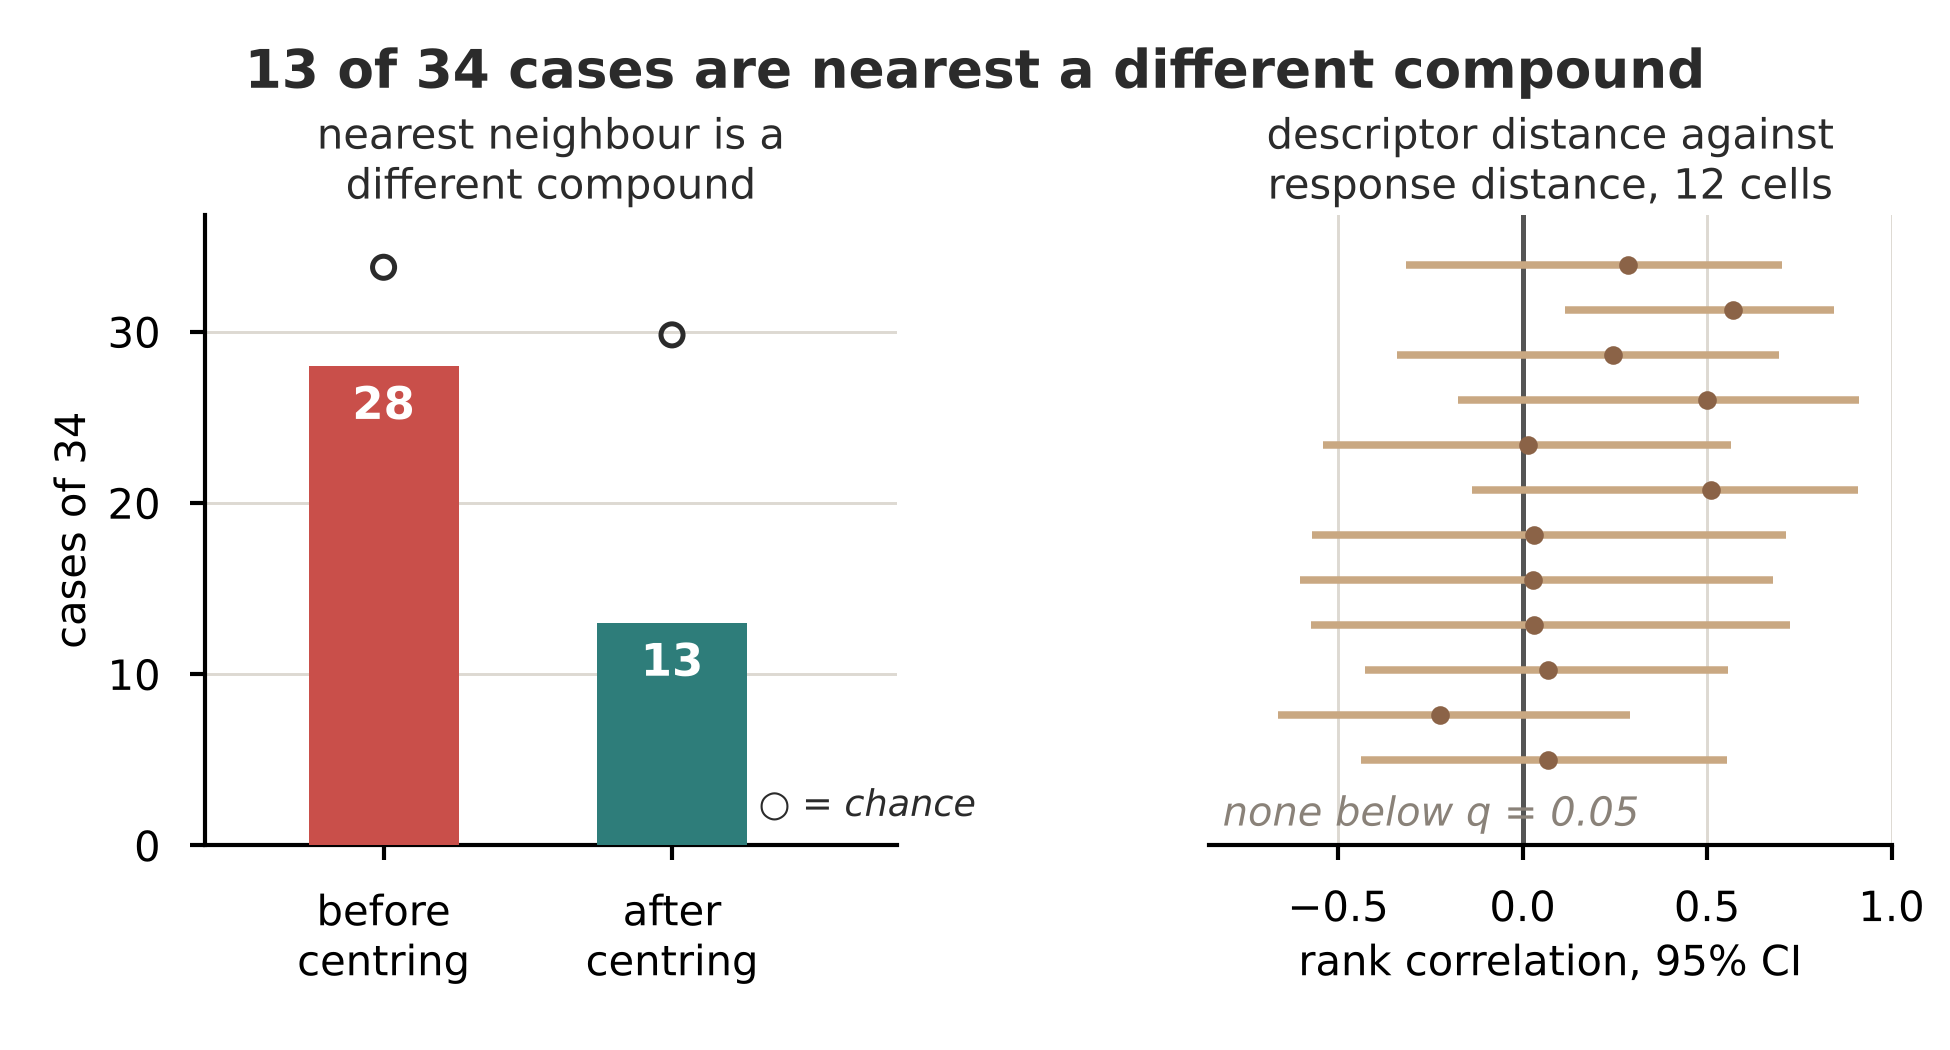
\includegraphics[width=3.25in]{toc_acs.png}
\end{tocentry}

\begin{abstract}
\noindent
Chemical warfare agent detection is developed almost entirely on simulants,
compounds accepted as agent-like and safe. We asked what that acceptance rests
on. No incumbent carries a public designation validating a detection response
against an agent's: one is designated for filter breakthrough, one in a training
patent that fixes a volatility window and asks for a detector response, the
third not at all, and we did not read the Army's selection procedure, which
bounds the claim. Exact permutation over every designation tested whether the
three sit closer to eleven agents than other non-agents, in structural and
GFN2-xTB electronic descriptor spaces and against a colorimetric sensor array.
On a thirty-five-compound panel no agent has a valid match and nothing is
significant; a twenty-eight-compound panel omitting five literature simulants
and two pesticides yields three matches and a nominal structural $p$ of 0.028
that no correction leaves significant and that rises to 0.350 when four
compounds our own source names beside an incumbent join the pool. Moving labels
moves the answer, and not in one direction: 0.630 becomes 0.745 or 0.00075
with how many move. Volatility, the axis the criterion names, gives the one
nominal value under 0.05 ($p = 0.0206$), but it tracks how widely the three
cover that axis, not how close they sit; read two-sided it is 0.182. The
corrective is a declaration, not a replacement compound: a defensible claim must
name the measurement it rests on and fix panel, space, statistic, comparison
pool and weighting in advance.
\end{abstract}

\section{Introduction}

Work on detecting chemical warfare agents (CWAs) is rarely done with CWAs.
Outside a few licensed facilities, sensor arrays, sorbents and sampling
protocols are developed and published using simulants: compounds chosen to
behave like an agent while being safe in an ordinary laboratory. The choice
therefore sets a ceiling on what a published detection result can be taken to
mean, and it is made by convention rather than by measurement.

The dependence is structural. Reactivity and sensing chemistry are established
on surrogates and extrapolated to agents in the standing reviews of agent
destruction and detection \cite{kim2011,jang2015}, in the recognition chemistry
developed for nerve agents \cite{royo2007,sambrook2013,eubanks2007} and in the
colorimetric sensor-array lineage much field instrumentation descends from
\cite{rakow2000,askim2013}, so the compounds an array is characterised on are
inherited rather than fixed by the chemistry. How rare the alternative is shows
in the exception: running a 73-indicator colorimetric array against fourteen
authentic agents was, the authors recorded, novel to their knowledge
\cite{davidson2020}. Our own work sits on both sides
\cite{hazref,multiplexref,ondeviceref,group3ref}, and what a simulant is for
differs by subfield \cite{bartelthunt2008,mondloch2015,ebeam}, but the inference
always runs from simulant to agent on a resemblance argument.

The convention is property matching. A recent critical review of liquid,
low-toxicity simulants states the criterion plainly, align hydrophobicity,
volatility and solubility with the agent's, and describes the simulants it
assesses as presenting minimal toxicity risks \cite{webb2025}. That review
covers liquid-phase sampling, but the same criterion underwrites vapour-phase
detection, where the quantity of interest is a chemical response.

Two assumptions are built into this practice, and both are testable. The first
is that resemblance in structural and physicochemical descriptors implies
resemblance in the property a sensor reports. For adsorption in metal--organic
frameworks it has been examined directly: four common simulants and two nerve
agents simulated across 2969 frameworks reproduced agent adsorption behaviour
only partially \cite{agrawal2018}. The analogous question for the electronic
properties governing a chemical response has not been asked. A cheminformatic
attempt at the selection problem predates this one. Lavoie et al.\ applied
pharmaceutical similarity search to simulant identification, seeking compounds
close to the agents but less toxic \cite{lavoie2011}. What we add is that
the compounds the detection literature settled on were not reached by it or by
any comparable procedure we could find. The second assumption is that a simulant
is safe, usually supported by the absence of an agent-class hazard label rather
than by a toxicity value, which is the practice in detection; the
human-decontamination literature instead screens against toxicity explicitly,
one review discounting 78 of 171 chemicals on the risk to volunteers
\cite{james2021}.

Both can be checked against measurements that already exist: the electronic
structure of small molecules is accessible at semi-empirical tight-binding cost
\cite{gfnxtb2017,bannwarth2019}, and acute inhalation toxicity has been derived
by a formal regulatory process for several hundred chemicals including the
agents themselves \cite{watson2006}. We ask where simulants and agents sit
relative to one another, how much of that answer is fixed by the data rather
than by the analyst's choice of panel, space and statistic, and whether the
incumbents are safe on a value or on an absence. The first question took a
different shape than we expected: a difference we found between descriptor
spaces survived neither extending the panel, nor correcting for the number of
statistics computed, nor removing a descriptor that was an exact function of two
others. That earlier reading is reported below alongside what the data support,
because how a nominal result of this kind arises is part of what a reader of
this literature needs.

The premise is not ours alone, and the nearest recent work states it. Lawrence
and Van Houten set out a systems-engineering method for developing simulants,
with stakeholder requirements, a down-selection against stated criteria, a
property database and a validation step, introduced against the observation that
simulants have more often been adopted for convenience than designed
\cite{lawrence2025simulants}. We take that as given and ask the retrospective
question their method does not: what the compounds already in service rest on,
and how much of any answer is fixed by the data rather than the analyst. Theirs
is a procedure for the simulants a programme will build; ours is an audit of the
three the optical sensing literature already uses, and a measurement of how far
its verdict moves when panel, space, statistic, comparison pool or weighting is
chosen differently. The two meet at the same corrective and overlap in neither
what they examine nor what they report.

\paragraph{Dual-use statement.} Throughout, the optimisation direction is
fixed: fidelity to the detection-relevant properties is to be maximised while
phosphorus electrophilicity, acetylcholinesterase reactivity, alkylating
capacity and predicted mammalian toxicity are to be minimised. No analysis here
ranks compounds by predicted mammalian toxicity, and we did not extend the
toxicity model of Supporting Information Section~\ref{S-sec:qsar} to the
organophosphorus class, because a model predicting mammalian lethality for
structures not yet made would invert the direction of the work; that a safety
model can be run in reverse is not hypothetical \cite{urbina2022}, and how much
of such a method to disclose is a live problem \cite{cbrndisclose}. Mechanistic
modelling of organophosphorus lethality is established and separately published,
including by the present authors \cite{qsarld50}; what is withheld is its use as
a design objective over novel structures, not the literature's existence.
Supporting Information Section~\ref{S-sec:dualuse} takes every analysis in this
paper in turn and states what it orders, over which compounds, and why its
release adds no structure-activity information the text does not already give.

\section{Methods}

\subsection{Compound set and the two panels}
\label{meth:panels}
Eleven authentic agents are common to both panels: sarin GB, soman GD, tabun GA,
cyclosarin GF, VX, sulfur mustard HD, lewisite~1 L, hydrogen cyanide AC,
cyanogen chloride CK, phosgene CG and chloropicrin PS. Three compounds are
treated as the incumbent simulants: DMMP, dichloromethane and dipropylene glycol
monomethyl ether (DPGME). We call them incumbent rather than designated because
the word reports usage and not standing: they are what the sensing literature we
surveyed runs its arrays and sorbents against, and that usage is thin for two of
them, resting on one metal-oxide sensor study for dichloromethane
\cite{lee2011sno2} and on a training patent for DPGME
\cite{seitzinger2006simulant}, so a different survey could return a different
three. Section~\ref{res:docs} reports what searching for a designating
instrument returned.

The two panels differ only in the non-agent pool, and the difference is the
point. The twenty-eight-compound panel adds fourteen interferents and solvents
routinely reported in sensor-array selectivity panels. The thirty-five-compound
panel adds, to those, five further compounds used as simulants in the sensor,
sorbent and decontamination literature (diisopropyl fluorophosphate DFP, diethyl
chlorophosphate DCP, diethyl cyanophosphonate
DCNP\cite{lee2021tabun,jang2014tabun}, 2-chloroethyl ethyl sulfide CEES and
methyl salicylate), classified as simulants rather than as interferents, and two
organophosphorus pesticides, dichlorvos and malathion. We class the pesticides as
interferents, and that classification runs against three of our own sources
rather than with them, which Supporting Information
Section~\ref{S-meth:panelsi} sets out; we kept it because those five are used to
stand in for an agent in detection work and these two are not, which is a
distinction about use rather than chemistry, and
Section~\ref{res:panels} reports how sensitive the result is to exactly this
kind of decision. The thirty-five-compound panel is the primary one, because a
comparison asking whether three compounds are close to the agents while
excluding the obvious alternatives is not a test of those three; the
twenty-eight-compound panel is reported throughout with equal numerical detail,
because what it shows beside the larger one is the paper's result. All class
labels were read from a single canonical table and never assigned by hand.

Panel, space, statistic, comparison pool and descriptor weighting were not
fixed before the analysis was run, and this paper's conclusion is that they
should be; we state
that here so the standard we recommend can be applied to the work recommending
it. The thirty-five-compound panel was built, and designated primary, after the
twenty-eight-compound result was in hand, which is the same post hoc choice this
paper catalogues in others. Supporting Information
Section~\ref{S-meth:prespec} sets out each of the five choices, when it was
made and what the alternative gives, with the block-weighting alternative in
Table~\ref{S-tab:blockbalance}, the per-panel match counts in
Table~\ref{S-tab:si-ascl3} and the relabelling null in
Table~\ref{S-tab:premisenull}.

\subsection{Descriptors and descriptor spaces}
Structural and physicochemical descriptors (51 after excluding run metadata)
were computed with RDKit \cite{rdkit} from canonical SMILES; electronic
descriptors with GFN2-xTB \cite{bannwarth2019} in the gas phase, since
vapour-phase response is the property of interest. Three spaces are compared:
structural, electronic and merged. Interpretable descriptors were used in
preference to a substructural fingerprint, because the quantity of interest is
position along named physical axes rather than a similarity score. Supporting
Information Section~\ref{S-meth:descriptors} gives the descriptor list, the
conformer treatment, the electronic protocol and the correlation and
exact-dependence filters that leave 38 structural coordinates on the primary
panel and 35 on the twenty-eight-compound one. Distances are Euclidean on
standardised descriptors, normalised by the median nearest-neighbour separation
of the panel in hand, so a normalised distance is comparable within a panel and
not between panels.

\subsection{The volatility axis}
\label{meth:vol}
The criterion the field states for simulant choice names volatility explicitly
\cite{webb2025}, and the electronic descriptors above are computed in the gas
phase for the same reason, so vapour pressure is carried as a third space in its
own right rather than left implicit. It is one-dimensional: a single measured
quantity, $\log_{10}$ of the vapour pressure in mmHg, with no filtering or
weighting to choose. Values were taken under a three-tier rule fixed before collection, preferring a
25~$^{\circ}$C value from a vapour-pressure compilation or dedicated measurement
report, then a 25~$^{\circ}$C government-handbook value, then the nearest
available temperature recorded with that temperature; twenty-four of the
twenty-eight compounds take the first tier, and one further value is marked as
extrapolated rather than measured by its source. Supporting Information
Section~\ref{S-meth:vol} gives every value with its source, its tier and the
adjudication where sources disagree. The axis is available on the
twenty-eight-compound panel only: no measured vapour pressure is recorded in
the source we fixed in advance for
diethyl chlorophosphate or for diethyl cyanophosphonate, so the thirty-five
compound panel cannot carry it.

\subsection{Nearest-neighbour comparison and permutation test}
\label{sec:perm}
For each authentic agent we recorded the distance to the nearest incumbent
simulant and to the nearest interferent. With fourteen interferents against
three simulants the minimum of fourteen draws is smaller than the minimum of
three by construction, so a paired test of the two distances is confounded by
group size. We therefore enumerated all ways of designating three of the
non-agents as simulants, computed the same statistic for each, and report the
rank of the actual designation as an exact $p$-value: $\binom{24}{3}=2024$
designations on the primary panel and $\binom{17}{3}=680$ on the
twenty-eight-compound one. The null expectation for ``an interferent is closer''
follows from the group sizes alone and is 9.63 of 11 on the primary panel and
9.06 on the smaller one. The hypothesis is directional, so the reported $p$ is
one-sided; the choice is consequential, and Supporting Information
Section~\ref{S-res:paneldetail} gives both two-sided conventions, under one of
which the structural value sits outside a conventional threshold. This is the
first of the analyst choices catalogued in Section~\ref{res:panels} and the only
one with a defensible default.

How the comparison pool is rebuilt under each relabelling is a further choice,
and the one we were slowest to declare: we take it to be every non-agent the
labelling did not designate, and two other readings give 0.054 and 0.160 in the
structural space against the 0.028 reported here (Supporting Information
Section~\ref{S-meth:prespec}).

\subsection{Match criterion}
\label{meth:match}
Nearest-neighbour rank alone is not sufficient: in the 38-dimensional merged
space of the twenty-eight-compound panel a ``nearest'' simulant at a distance of
11.70 is not a match. We therefore normalised each distance by the median
nearest-neighbour distance of the same space and define a valid match as a
normalised distance $\le 2$ together with a distance smaller than that to every
compound outside the designated set. The threshold is a convention; the second
condition is not.

The comparison set named in the second condition can be read three ways and the
reading changes the count, so we declare ours: every compound that is neither an
authentic agent nor a designated simulant, twenty-one compounds on the primary
panel and fourteen on the twenty-eight-compound one. The two alternatives, and
the count each gives on each panel, are in Supporting Information
Section~\ref{S-meth:failaudit}; the narrower of them raises the primary-panel
count from zero to three only by removing the five literature compounds from the
comparison, which is the panel-composition effect of Section~\ref{res:panels}
acting on the criterion rather than on the chemistry. The criterion is a
statement about proximity in this descriptor space and nothing further. On the
primary panel the incumbent simulants fail the second condition for all eleven
agents, so the count there is zero at every threshold, including an unbounded
one.

\subsection{Reproducibility}
\label{res:repro}
All analyses are deterministic given the seed, which is 42 except where a
script records otherwise. The designation and Mantel permutation tests are
exhaustive. Seven analyses are sampled rather than enumerated, at between 1000
and 20000 draws each; Supporting Information
Section~\ref{S-meth:sampling} names them with their draw counts. Supporting Information
Section~\ref{S-meth:sampling} names the sampled analyses and the pinned version
of every library the pipeline uses
\cite{numpy2020,scipy2020,mckinney2010,matplotlib2007,rdkit,pyscf2020}.

One part of the descriptor table cannot be regenerated, and we state it here
rather than in the deposit alone. The three electronic coordinates come from a
GFN2-xTB binary whose version was not recorded when the cache was built, so
those columns rest on the deposited cache rather than on a reproducible
calculation, as do the five further columns the same binary produced, of which
one is an algebraic function of the orbital energies and four are independent
outputs; only the three enter any distance reported here; the gate
\texttt{build\_descriptors.py --verify} regenerates the fifty-three columns
RDKit can rebuild and exempts the rest by name.

\begingroup\sloppy
The deposit also carries two consistency harnesses, and their scope is narrower
than their names suggest. \texttt{verify\_consistency.py} locates each
registered quantity in the manuscript by a regular expression and compares it
with the generator output, reporting both what it matched and what it could not
locate, the second not being zero. A second harness
(\texttt{test\_verify\_consistency.py}) injects defects and checks that the
first catches them. Neither checks a claim the
manuscript makes about a document, and neither is a substitute for reading the
sources.
\endgroup

\section{Results}

\subsection{What the designating documents say, and for which measurement}
\label{res:docs}

Searching for an instrument that designates the three incumbent compounds as
chemical warfare agent simulants, we found that two carry documented
designations for purposes other than the one they now serve and the third
carries none. Supporting Information Table~\ref{S-tab:designations} grades every
designation we located by what its document does rather than by how
authoritative it looks, with the source URL and search date for each. Two of the three
we located for DMMP concern transport through a barrier: canister and cartridge
filtration against GB and HD in a NIOSH respirator programme
\cite{niosh2002simulant}, a document that also states its simulant information
is not a recommendation of any simulant, and fabric penetration against VX in
the Man-in-Simulant Test assessment \cite{nrc1997mist}. The third is the US
Army training-composition patent that also designates DPGME
\cite{seitzinger2006simulant}, and it is the one instrument of the three that
names a property rather than a barrier. Its granted claim 1(a) requires a
vapour-generating component ``having a vapour pressure of from about 0.1 to
about 30 mm Hg at 25$^{\circ}$C which is present in an amount sufficient to be
detectable by a vapour detection apparatus'', and claim 3 lists twenty-three
admissible components, dimethyl methylphosphonate and methyl salicylate among
them. The property it constrains is volatility, which is the axis
Section~\ref{res:vol} finds the designation is not indistinguishable from
chance on. What it does not do is compare the response it asks for with an
agent's: the specification asserts that the vapour characteristics are
comparable to G and H agents and names ion mobility, infrared and surface
acoustic wave detectors, but offers no measurement of an agent beside the
simulant and rests its preference for DPGME and methyl salicylate on years of
prior use as simulants. The designation fixes a volatility window and validates
that an instrument reacts; it does not validate that the instrument reacts as it
would to the agent. For dichloromethane we
found no designating document of any kind, and it is present in this role only
in the research literature \cite{lee2011sno2}.

A negative claim about documents is only as good as its scope, and ours has a
hole in it which is the most important document of all. TOP 08-2-196,
\emph{Simulant Selection for Laboratory, Chamber, and Field Testing}
\cite{top082196}, is the Army's procedure for exactly this question and we have
not read it. Its current revision carries a Defense Technical Information Center
accession and a full-text address in that agency's public repository, so the
document is reachable in principle; our own attempts to retrieve it failed, the
last of them on 14 November 2026, while that repository was under maintenance. What we know of its
role comes from TOP 08-2-188 CN1, which defers simulant selection to it
\cite{top082188} and itself states a detection criterion rather than a barrier
one, that the simulant ``should produce a signature signal similar to the one
from the threat analyte''. The claim is therefore bounded by a document we did
not read rather than by one that does not exist, and the literature we did read
is listed in Supporting Information Section~\ref{S-res:searchscope}: among those
instruments the three compounds carry no designation validating a detection
response against an agent's, and we cannot say that no such instrument exists.

The observation that follows is that a designation is specific to a measurement,
so a compound chosen because it breaks through a carbon bed like sarin has been
validated for adsorption and not for an optical or electrochemical response.
That holds even where the instrument is clearest: methyl salicylate carries a
consensus standard fixing the measurement as vapour penetration of a protective
ensemble \cite{astmf2588}, yet the National Academies assessment of that
programme records that its selection ``was based on its historical use as an
agent simulant'' and that the assumptions behind it ``have not been tested''
\cite{nrc1997mist}.

\begin{figure}[tp]
\centering
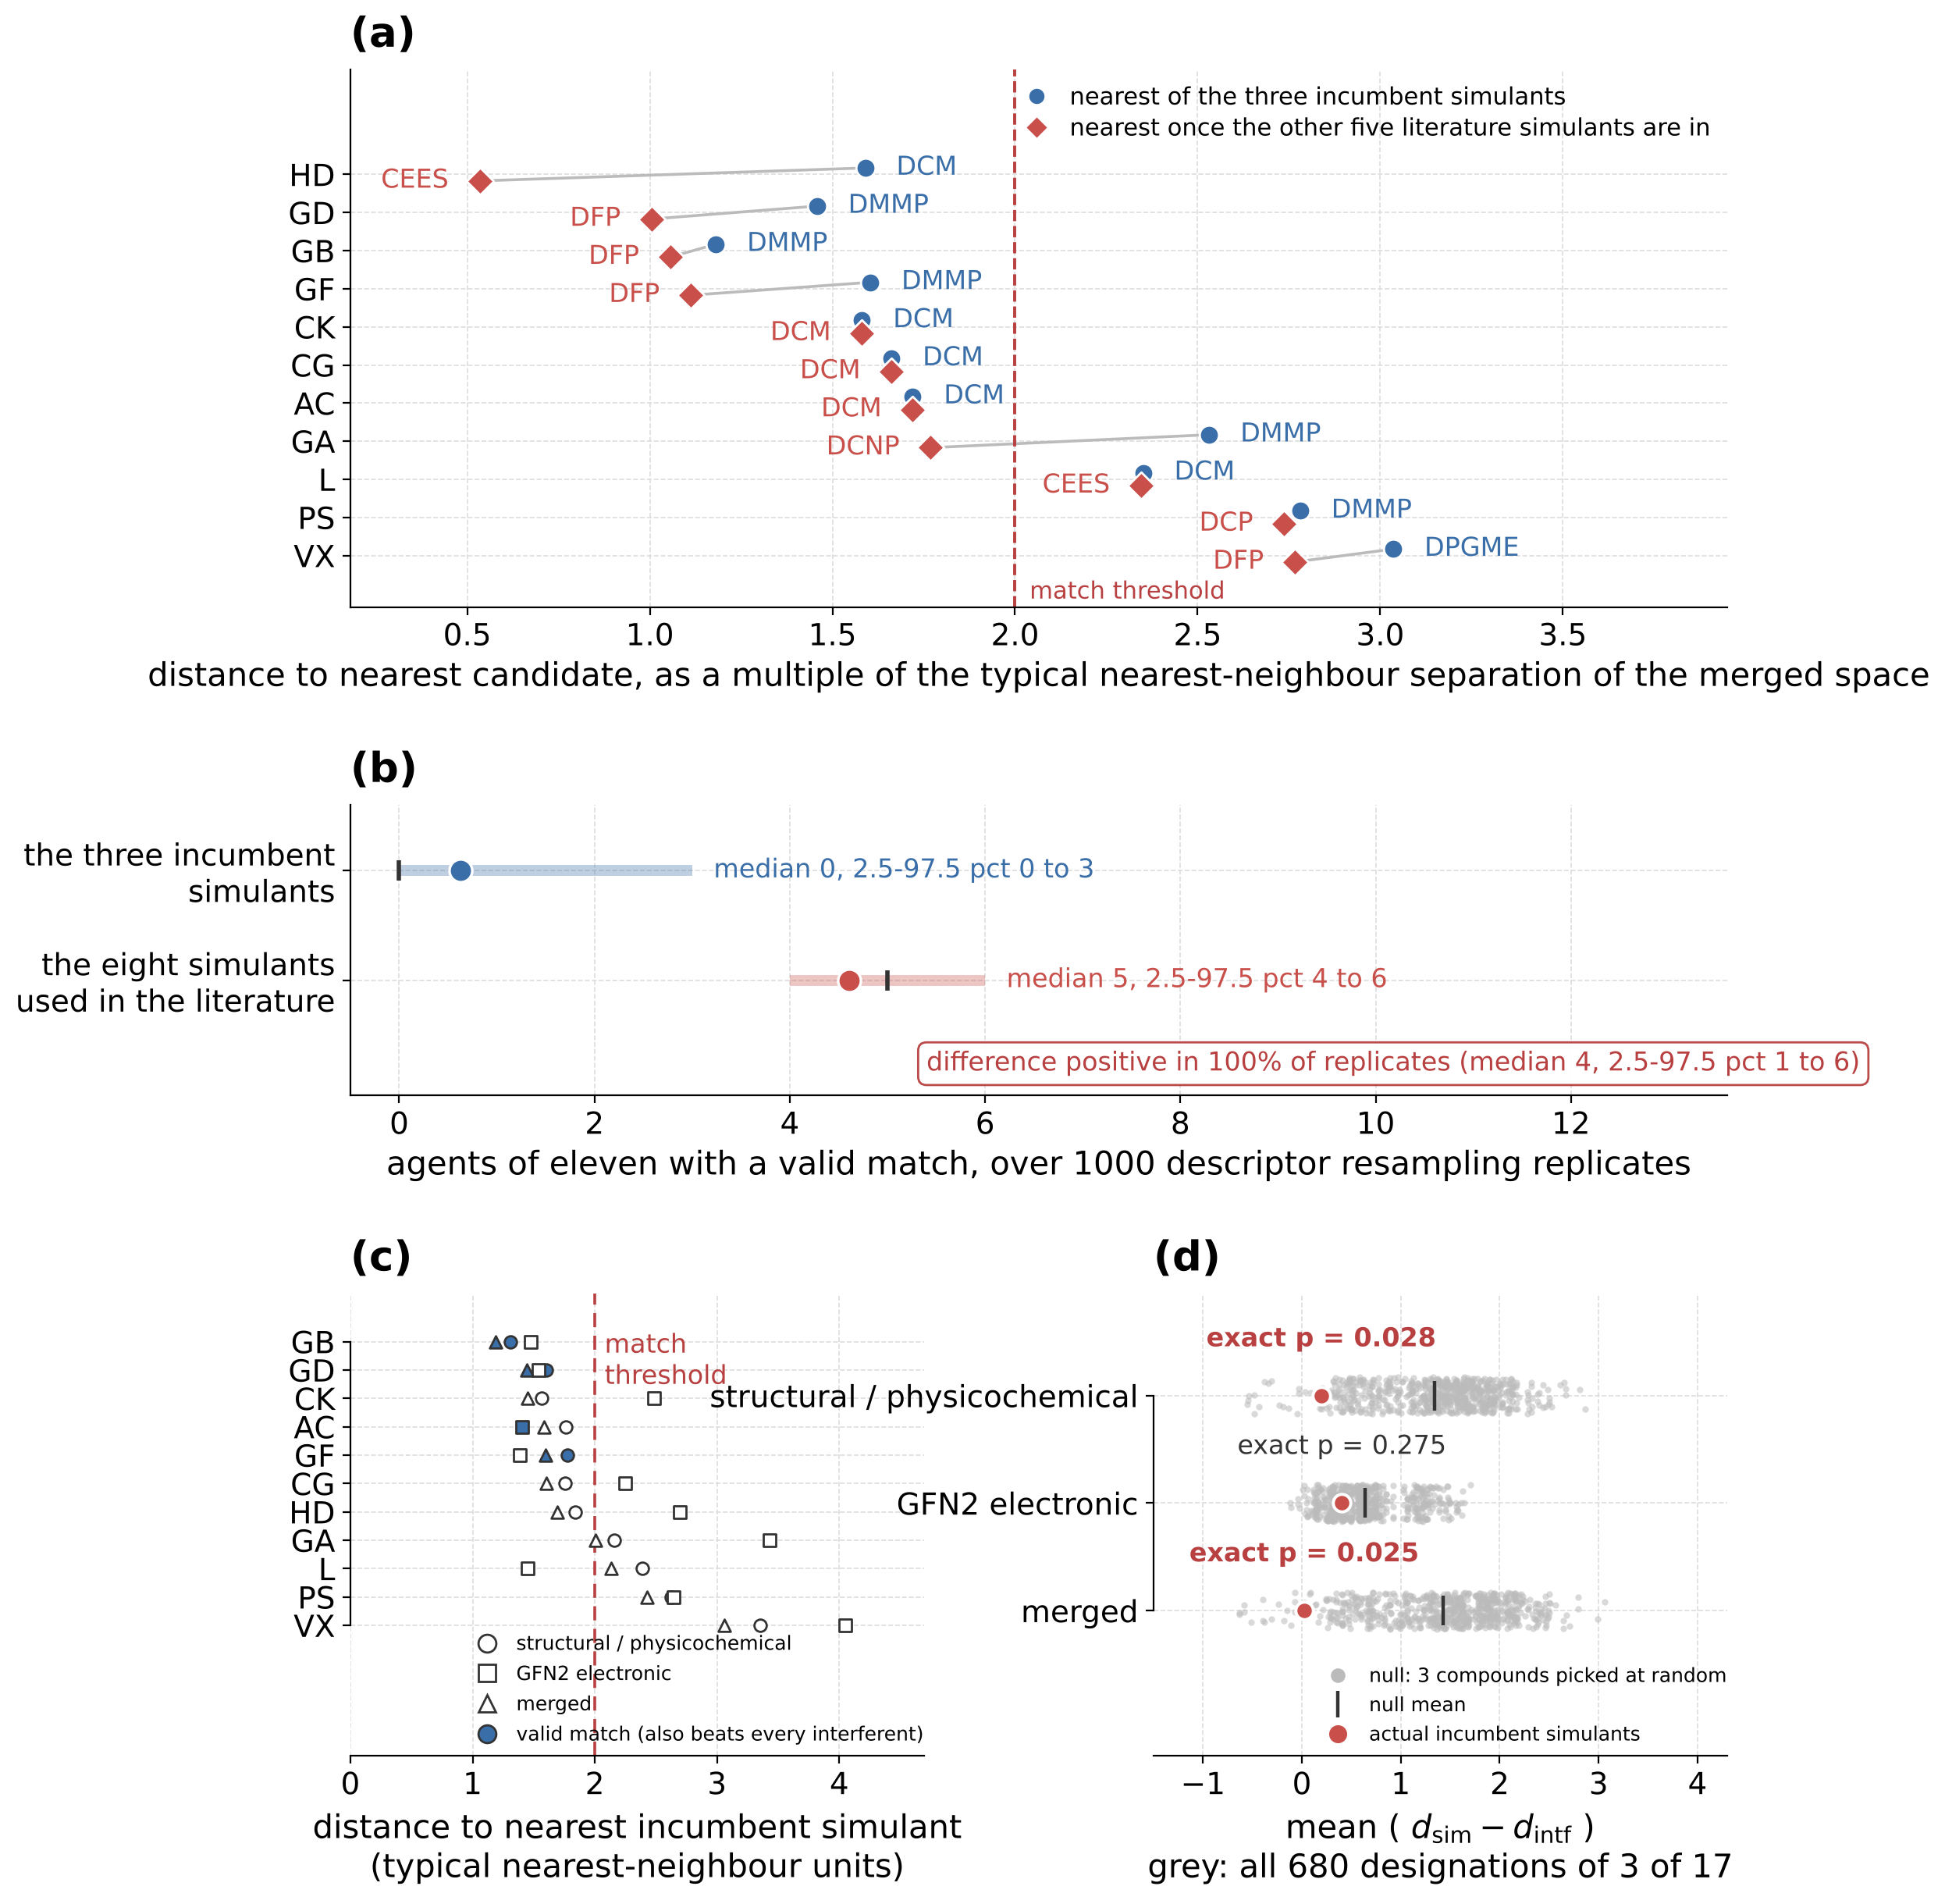
\includegraphics[width=0.79\textwidth]{Fig_main.png}
\caption{What the comparison contains decides the answer. Distances are
normalised by the typical nearest-neighbour separation of the space in hand,
and a valid match requires a normalised distance below the dashed threshold
\emph{and} a distance smaller than that to every compound not designated a
simulant. (a) Thirty-five-compound panel, merged space: nearest incumbent
simulant (circles) and nearest candidate once the five literature-used
compounds are admitted (diamonds). (b) Matched agents over 1000
descriptor-resampling replicates; circles means, rules medians, bars the 2.5th
to 97.5th percentiles. (c) Twenty-eight-compound panel, the three spaces;
filled markers are valid matches. (d) Exact permutation null for that panel
over all 680 designations, actual designation marked, mean-difference statistic
(Benjamini-Hochberg over the eighteen tests, 0.163). (e) Volatility axis, in
$\log_{10}(P/\mathrm{mmHg})$; the one pairing inside the criterion, soman to
DPGME, lies 0.0107 decades apart. Section~\ref{res:panels} and Supporting
Information Sections~\ref{S-meth:dboot} and~\ref{S-meth:vol} give the
constructions.}
\label{fig:main}
\end{figure}

\subsection{What the comparison contains decides the answer}
\label{res:panels}

On the thirty-five-compound panel, no authentic agent has a valid match to an
incumbent simulant. The mechanism is panel composition rather than chemistry,
and it is not the one our earlier version reported: the compounds did not become
less faithful, but diisopropyl fluorophosphate is present and is nearer to
sarin, soman and cyclosarin than DMMP is, and the criterion requires a simulant
to be nearer than every compound not designated one (Figure~\ref{fig:main}a).
Admitting the five as simulants gives five matched agents of eleven, against
three on the twenty-eight-compound panel and zero on the primary one. The zero
does not depend on the threshold: no incumbent is the nearest non-agent compound
to any of the eleven agents, so the count stays at zero however far the
threshold is relaxed, and because zero is the smallest attainable count the
resampling comparison returns $p=0.479$, the smallest value it can ever return
and a comparison that cannot reach significance whatever the data. Resampling
the descriptors leaves that contrast in place (Figure~\ref{fig:main}b), and
Supporting Information Section~\ref{S-res:paneldetail} gives the intervals, the per-agent
reliabilities, which reverse what the point estimates suggest, and the dimension
and subspace controls.

The exact permutation tests over the four panel and designation constructions
are in Supporting Information Table~\ref{S-tab:ablation}, in full rather than
selected from, because the pattern across the cells is the finding; the two
relabelling enumerations reported later in this section are in the deposit
under their own names. On the primary panel no test reaches
nominal significance in any space under any statistic, while classing the five
literature compounds as simulants recovers two nominal values below 0.05, so the
difficulty is not that the test cannot detect anything here. On the
twenty-eight-compound panel the incumbents beat random compounds under one of
six statistics in the structural space and three of six in the merged space, and
correcting for the number of times we looked removes almost all of it: over the
six accounting schemes of Supporting Information
Section~\ref{S-meth:multiplicity} the eighteen-test family leaves that result at
0.163 and the closest any scheme brings it without crossing is 0.077. Had the
mean difference been named in advance as the single statistic it would survive
at $q=0.042$, but we computed six and chose among them after seeing them,
which is the circumstance the correction exists for, and that declaration is one
nobody in this literature makes.

How many labels are moved decides the direction, and not monotonically. Classing
dichlorvos and malathion as simulants and changing nothing else makes the result
worse, not better: the smallest Benjamini--Hochberg value over the same eighteen
tests moves from 0.630 to 0.745. Classing all seven of the undesignated
organophosphorus and literature compounds as simulants gives a smallest nominal
value of 0.00006 and a corrected 0.00075, the only one of the four
configurations in Supporting Information Table~\ref{S-tab:family} that survives
all six accounting schemes. Neither relabelling is arbitrary, and on one we
correct ourselves: we called the two pesticides compounds nobody uses as
simulants, which is wrong for malathion, which the NIOSH document lists in a GB
simulant column with breakthrough times \cite{niosh2002simulant}.

The cheapest relabelling of all needs no new compound and no new citation. Two
of our three incumbents come from one metal-oxide sensor study, which assigns
four compounds to four agent classes in a single sentence: acetonitrile to blood
agents, DMMP to nerve agents, DPGME to blister agents and dichloromethane to
pulmonary agents \cite{lee2011sno2}. We took three of the four and left
acetonitrile in the comparison set, where it is the compound that blocks sarin,
soman and cyclosarin in the electronic space. Moving that one label, on the
authority that already supplies two of our incumbents, takes the
twenty-eight-compound result from a corrected 0.163 to 0.023 and the matched
count from three to five, and on the thirty-five-compound panel moves 0.630 to
0.421 (\texttt{outputs/acetonitrile\_panel.json}). We did not make that move
when we built the panel and did not record not making it; it is reported rather
than adopted, because we have no ground to prefer the four-compound reading. An
analyst with a citation in hand can move a defensible number of labels and land
anywhere between 0.745 and 0.00075, and the practice records neither that labels
were moved nor how many.

What those nominal results carry is narrower than it sounds, and the sign of
the statistic says so. Four of the eighteen cells fall below 0.05 before
correction, one in the structural space and three in the merged one, and the
smallest is the merged mean difference at 0.025 rather than the structural
0.028 the abstract quotes. The observed mean difference in the structural space
is $+0.195$: the designated simulants are on average
\emph{further} from the agents than the nearest compound outside the designated
set. What the test detects is only that they are less far than a triple drawn at
random from a pool chosen because its members are not like the agents, and
against that reference class one organophosphorus compound is close to
sufficient.

One addition to that pool removes the value, and the compounds to add were
named in our own evidence. The respirator document we rely on for DMMP's single
designation lists eleven candidates for its permeation study, and four stand in
that list beside DMMP itself: diisopropyl methylphosphonate, diethyl
ethylphosphonate, triethyl phosphate and di-n-butyl sulfide. None is on either
panel, and we did not record the decision to leave them off, which is the
comparison-pool freedom this paper asks others to fix, taken once more and in
our own favour. Admitting the four with the designated set unchanged takes the
nominal structural value from 0.028 to 0.350 and the valid matches from three to
one on the twenty-eight-compound panel, and from 0.351 to 0.424 with no match
either way on the primary one. Nothing survived correction before the change;
what does not survive the change is the nominal value the abstract quotes.
Diisopropyl methylphosphonate stands nearer than any incumbent to soman, to
cyclosarin and to VX, and di-n-butyl sulfide nearer to sulfur mustard than
dichloromethane, leaving sarin the only matched agent, which is the mechanism
diisopropyl fluorophosphate supplies on the primary panel. We report the
extension rather than adopt it, and it reaches the structural space only,
because the electronic coordinates would need the semi-empirical binary whose
version we did not record (Section~\ref{res:repro}). Supporting Information
Section~\ref{S-meth:niosh} gives the structures, the distances agent by agent
and the coordinates the filters exchange when the pool grows.

\subsection{How many agents have a valid simulant depends on the panel}
\label{res:match}

Figure~\ref{fig:main}c and Supporting Information Table~\ref{S-tab:match} give,
for each agent on the twenty-eight-compound panel, the nearest incumbent
simulant as a multiple of that space's typical nearest-neighbour separation,
and Figure~\ref{fig:main}d the permutation null behind the nominal value. Sarin
(1.187), soman (1.446) and cyclosarin (1.594) are matched, all three by DMMP;
tabun at 2.004 and VX at 3.057 are not. Tabun misses the threshold of 2 by
0.004, and we flag that rather than report the count as firm: an earlier version
of this analysis, which retained a structural coordinate that is an exact
function of two others, put tabun at 1.9948 and counted four matches instead of
three. A count that moves when a redundant coordinate is removed should be read
as marginal.

The count is stable but not invariant. In the merged space the matched set runs
from \{GB, GD\} at a threshold of 1.5 to \{GB, GD, GA, GF\} at 2.5 and 3.0, tabun
entering only once the bar passes its value of 2.004, and over the thresholds
tested the count does not exceed four of eleven in any space
(\texttt{outputs/threshold\_sweep.json}). The electronic space behaves
differently: there the count is one at every threshold tested, hydrogen cyanide
matched by dichloromethane at 1.407, because acetonitrile sits closer to sarin,
soman and cyclosarin than DMMP does and all three fail the threshold-free
condition outright. Two things stop that contrast from reading as chemistry, and
both are set out in Supporting Information Section~\ref{S-res:dimdetail}: the
same normalised threshold is not equally strict across spaces of different
dimension, admitting 14.8 per cent of all pairs in the electronic space against
42.1 per cent in the merged one, and the electronic coordinates are
semi-empirical by a margin larger than the spacing they have to resolve.
Rebuilding the space at the density-functional level moves the matched count
from one to five. Crossing the threshold-independent choices instead gives
twenty-five cells in which the matched set takes seven distinct values, and five
agents have no valid simulant in any of them (Supporting Information
Section~\ref{S-meth:failaudit}).

The dependence on the panel is sharper than the dependence on the threshold, and
Section~\ref{res:panels} gives it: on the thirty-five-compound panel the merged
space returns no valid match for any of the eleven agents, and admitting the
five literature compounds as simulants gives five of eleven, more than the
incumbent set achieves on either panel. VX remains unmatched in every panel and
space we examined. We draw no conclusion that the field should switch compounds,
because the five were not selected by any procedure we can inspect either. What
the comparison establishes is narrower: the statement ``three of eleven agents
have a valid simulant'' is true of one panel, false of a second, and replaced by
a different list on a third, which is the same instability the permutation tests
report and not an independent finding.

\subsection{The axis the stated criterion names}
\label{res:vol}
Volatility is the one axis the stated criterion names that is not a descriptor
we chose, and the one axis on which the test returns a nominal value below
0.05. Two readings of that value, set out below, take it back above 0.05. Two tests were registered in advance of it,
outside the family of eighteen reported above; only the first was reported in
the form registered for it, and Supporting Information
Section~\ref{S-meth:vol} gives both in full with every adopted vapour pressure
and its source.

The designation test repeated on the one-dimensional axis puts the incumbent set
fourteenth on the pre-specified statistic, a one-sided $p$ of 0.0206 over all
680 designations. Its registered form and its reported form are the same, so the
exemption from the eighteen holds for this one; corrected within the two tests
registered for this axis it stands at $q = 0.0412$. That registration is a
statistic named inside the script that computes it, with no external timestamp,
and Supporting Information Section~\ref{S-meth:vol} sets out what it is worth
and what the value becomes under wider families. It does not carry to the match criterion
(Figure~\ref{fig:main}e): the valid-match count returns one match at
$p = 0.4647$, pairing DPGME with soman across a gap smaller than the mismatch between the temperatures
at which the two vapour pressures were measured, so nothing rests on it. Three
of the eleven agents have an interferent nearer than any incumbent here as
well.

Two readings weaken that 0.0206, and both were ours to make. The three
descriptor spaces above are each reported one-sided and two-sided; this axis was
reported one-sided only, and under the two conventions used there it stands at
0.0412 and at 0.182, the second of which does not reach 0.05. What the statistic
responds to is the second reading. On a single axis the mean difference falls as
the designated set covers more of the axis, and across all 680 designations the
two are nearly one quantity, with a Spearman correlation of $-0.971$. The
incumbent three cover more of this axis than any other triple in the pool, so
0.0206 is largely a comparison against triples covering less of it; held against
triples of comparable coverage it rises to 0.326, 0.203 and 0.101 at the top
twentieth, tenth and fifth of that distribution. Decomposing by size says the
same: DPGME alone is the best of the seventeen singles and dichloromethane the
worst, dichloromethane with DPGME is the best of the 136 pairs at 0.0074, and
the incumbent triple stands fourteenth of 680 where DMSO with DPGME and
dichloromethane stands first. The axis supports that three compounds spanning it
beat a triple drawn from a pool spanning less, not that these three were chosen
well for it. Supporting Information Section~\ref{S-meth:vol} gives the ranking
at each size and the coverage ladder.

The second test asks whether distance on this axis tracks the colorimetric
response the array recorded, and here we report against ourselves. The form we
registered combined the exact Mantel value of every evaluable cell in one Fisher
step. It returned $p = 0.0809$ and was withdrawn the same day for a per-channel
form under which the smallest adjusted value reaches $q = 0.0430$, in the
reflectance channel, while the ultraviolet channel does not. The replacement has
a reason, in that two channels of one plate are not independent, but it was
chosen after the result of the form it replaced was known, so it is post hoc and
carries no exemption from correction. Two further facts bear on it, both in
Supporting Information Section~\ref{S-meth:vol}: we drew the two-channel family
ourselves and the direction of that choice favours our own result, the four
cells read as one family giving 0.1389; and the only cell under 0.05, at
$p = 0.0458$, comes from the plate that carries no simulant. On the form we
registered, this axis reports no agreement either.

\subsection{What the two premises survive}
\label{res:measured}
\label{res:toxsummary}

Every argument above rests on descriptor distances, and the premise that one of
those spaces corresponds to what a sensor reports is tested in Supporting
Information Section~\ref{S-res:arraydetail} against measured colorimetric
response for twelve compounds. That response is not new here: it is taken from a
29-component array reported in earlier work from this laboratory
\cite{hazref,multiplexref,group3ref}, and those exposures were acetonitrile
solutions at matched molarity, not vapour, which bounds what any of this
establishes about a vapour-phase response. It does not resolve the question:
three of twelve cells reach a nominal $p<0.05$ and disagree on a space,
correcting over the twelve leaves 0.117, all three lie in the plate set
containing no simulant, and the six cells bearing on the premise are null while
the design detects only $|\rho| \ge 0.85$ after correction. The premise is
untested rather than supported, and every distance-based claim here inherits
that.

The criterion's second half, that compounds chosen on physicochemical grounds
present minimal toxicity risk \cite{webb2025}, was tested on the same panel
(Supporting Information Sections~\ref{S-meth:aegl}, \ref{S-res:safety},
\ref{S-sec:qsar} and \ref{S-res:h1}). The two incumbents differ in how well
documented they are and not only in how hazardous: dichloromethane carries an
Acute Exposure Guideline Level at the 96th percentile of a 207-compound pool,
although that value is an Interim one rather than a Final one, while DMMP is
absent from the list altogether and the Environmental Protection Agency
declined to derive an inhalation reference concentration for it. What DMMP does
carry is weaker and differently derived, and Supporting Information
Table~\ref{S-tab:registers} gives every register entry we located so that the
scope of that negative is visible. A model cannot fill the gap: a random forest trained on 230 AEGL chemicals
reaches $R^{2}=0.458$ and then predicts every one of twenty held-out military
agents safer than measured, by factors of 2.5 to 2600, while certifying fourteen
as inside its applicability domain. Fidelity and acute toxicity show no
detectable monotonic association across the 207 compounds carrying both measured
axes (Spearman $r=+0.062$, 95\% CI $-0.077$ to $+0.199$).

\section{Discussion}
\label{sec:discussion}

The criterion by which low-toxicity simulants are chosen is stated clearly
enough to test \cite{webb2025}: align hydrophobicity, volatility and solubility
with the agent. What the practice does not state is what the chosen compounds
should be compared against, and that decides the answer. The mechanism is not a
story about fidelity: the identity of each agent's nearest incumbent is unchanged
between the panels, and for the three G agents on which the argument turns the
distances move by under one per cent, the one agent whose distance moves enough
to matter being tabun (Supporting Information Section~\ref{S-disc:detail}). What
the larger panel supplies is diisopropyl fluorophosphate. A designation defended
by a comparison that excludes the alternatives is not defended.

An earlier version built a thesis on the contrast between the
twenty-eight-compound structural cell and the electronic space. We withdraw it:
the cell does not survive its own family ($q = 0.163$), it sits at the 22.4th
percentile of 2000 arbitrary three-descriptor slices of the same block, and
rebuilding the electronic space at the density-functional level moves it from
$p=0.275$ to 0.0368 (Supporting Information Section~\ref{S-meth:dft}).

What remains is a claim about comparison rather than about chemistry. On the
primary panel we can establish neither that the incumbent simulants are closer
to the agents than compounds drawn at random nor the opposite; what we can
establish is that the compounds which would make the comparison informative were
not in it.

The volatility axis separates the two halves of that statement. It is the only
one of the three on which the designation is not indistinguishable from chance,
and that result stands on the form specified in advance for it; whether distance
along it tracks the colorimetric response the array recorded is a second
question, and the form specified for that one returns no agreement
(Section~\ref{res:vol}). Two independent lines land on that axis. A National Research Council
committee writing about detection put the requirement in 2003: an ideal simulant
would mimic every property but toxicity, that is never achieved, and simulants
for vapour-phase detection must approximate the vapour pressure of the agent
\cite{nrc2003standoff}. And the one instrument we found that constrains a
property rather than a barrier constrains this one, by a window of about 0.1 to
30 mm Hg at 25$^{\circ}$C (Section~\ref{res:docs}). The documentary record and
the permutation test agree on which axis carries the designation, and that is
the only agreement between them we found. An external check gives no support to the other two
axes. Davidson et al.~\cite{davidson2020} exposed a 73-indicator colorimetric
array to fourteen authentic agents alongside precursors, pesticides and
household chemicals, and their clusters are a measured grouping a descriptor
space can be scored against. Of the six compounds we could place in both,
neither our structural space ($p = 0.500$) nor our electronic one ($p = 0.350$)
separates the three they grouped with an agent from the three in their
weak-response cluster; with six compounds the smallest attainable value is 0.05,
so that is absence of support rather than refutation, and the comparison set is
itself a choice we made with incomplete information
(Section~\ref{S-meth:panelsi}). Their analytes were delivered neat into a
headspace while our plates received solutions at matched molarity, so the
agreement we report on the volatility axis is a correlation with response
distance and not evidence that vapour delivery produced it. The incumbent
designations are therefore supported in kind on the one axis the criterion names
and undocumented in degree, since that axis ranks the designation 316th of 680
on match count and the single match it yields lies inside a temperature
mismatch.

The documentary record explains how that arose, and it is not a story about
carelessness. DMMP was designated for a stated measurement, adsorptive
breakthrough on a filter bed, in a document that declines to recommend any
simulant and carries a draft marking, and it carried that status into sensor
development, where the governing
property is the response of a dye or an electrode rather than a breakthrough
time (Section~\ref{res:docs}). The absence is specific rather than general: a
safety-screened repository of candidate simulants exists \cite{james2021} and a
descriptor-based selection procedure was published fifteen years ago
\cite{lavoie2011}; what is missing is any route by which either reached the
compounds the detection literature settled on. Treating a validation as a
property of the compound produces a working set no descriptor space reproduces,
and Agrawal et al.~\cite{agrawal2018} reach the same place from the other
direction. The corrective is a declaration rather than a replacement compound:
which measurement a simulant was validated against, and a panel, space and
statistic fixed before it is tested for a different one (Supporting Information
Section~\ref{S-disc:detail}).

\paragraph{Limitations.} The documentary findings of Section~\ref{res:docs} rest
on public sources, and the scope of that search is stated there: the claim is
that no public instrument designates these three compounds for the use the
sensor literature makes of them, not that none does. Sensitivity depends on the
threshold applied: against a nominal 0.05 the test reaches that threshold once
the incumbents are moved 0.24 typical separations closer, against an observed
median deficit of 0.493, but correcting across the eighteen tests raises the
detectable effect to 0.72, above that deficit and above the deficit of eight of
the eleven agents, so at the corrected threshold the design has no power against
an effect of this size (Supporting Information Section~\ref{S-res:mde}). The
nine shape coordinates are algebraic functions
of three principal moments, a dependence the correlation filter misses; dropping
the seven derived ones takes the twenty-eight-compound valid-match count from
three to zero while the nominal structural value survives at 0.034 (Supporting
Information Section~\ref{S-meth:shape}). Regulator-derived acute inhalation
values exist for part of the panel only, and for DMMP only outside the
guideline-level list. One omission is systematic: probe chemistries for lewisite
are developed against arsenic trichloride \cite{lee2016lewisite}, in neither
panel. Supporting Information Section~\ref{S-disc:detail} gives the rest.

\section{Conclusions}

Simulant validity is not an intrinsic property of a compound. It depends on the
measurement the compound is meant to reproduce and on the comparison the claim
is scored against, and the practice of choosing chemical warfare agent simulants
records neither. DMMP was designated for filtration breakthrough, DPGME in a
training patent that fixes a volatility window and asks that a vapour detector
respond, and dichloromethane
carries no designating document; none of the three validates resemblance. The
test that would establish resemblance returns whatever the analyst's undeclared
choices imply, from a corrected 0.745 to 0.00075 on one panel according to how
many labels are moved, and the one axis on which the designation is
distinguishable from chance is the one the stated criterion names.

A simulant result should therefore name the measurement the compound was
validated against and the comparison set it was tested in, and should fix the
panel, space, statistic, comparison pool, weighting and treatment of
conformer-dependent
descriptors before the test is run; we add the last because a reproduction check
caught us not counting it. We propose no replacement compound, because proposing
one would repeat the error this paper is about.

\begin{suppinfo}
The Supporting Information is available free of charge at [DOI to be assigned].
It contains the descriptor construction and resampling procedure, the scope of
the documentary search, the panel and dimensionality controls, the full
permutation family and its accounting schemes, the measured colorimetric array
response, the acute toxicity axis with its interpolation and decoupling tests,
the structural filter and local reactivity analysis, the dual-use audit, and the
remaining limitations (PDF).
\end{suppinfo}

\section*{Author Contributions}
\textbf{Ku Kang:} conceptualisation, methodology, software, formal analysis,
investigation, data curation, visualisation, writing -- original draft.
\textbf{Jeongyun Kim:} formal analysis, investigation, validation.
\textbf{Miae Kim:} investigation, validation, writing -- review and editing.
\textbf{Doo-Hee Lee:} validation, resources, writing -- review and
editing, supervision. \textbf{Jin Yoo:} methodology, investigation,
validation, writing -- original draft. \textbf{Yoon Jeong Jang:} validation,
writing -- review and editing, supervision, project administration.

\section*{Notes}
The authors declare no competing financial interest.

\section*{Acknowledgement}
This research did not receive any specific grant from funding agencies in the
public, commercial, or not-for-profit sectors. During the preparation of this
work the authors used a large language model (Anthropic Claude) to assist in
drafting and editing prose and in writing and auditing the analysis, figure and
consistency-check scripts. No numerical result was produced by the model: every
value is read from the output of the deposited scripts. The authors reviewed and
edited all content and take responsibility for it.

\section*{Data and code availability}
\begingroup\sloppy
Descriptor tables, parsed AEGL values with sources, permutation distributions,
candidate tables, the EPA source document every toxicity value was parsed from,
and all analysis and figure scripts are in a public repository at
\url{https://github.com/bisu9082/simulant-designation-evidence}, and are also
provided with this article; the release tagged for this submission is the one
named \texttt{acs-submission-20261112}.
The descriptor cache is checked against the
code: \texttt{build\_descriptors.py --verify} rebuilds the fifty-three columns
RDKit can regenerate, halts if any fails or if any column outside the declared
exemption list goes unchecked, and exempts nine columns needing the xtb binary,
eight of them present on the twenty-eight-compound cache and unchecked. Those
include all three coordinates of the electronic space, so that space rests on
the deposited cache rather than a reproduced one.
Section~\ref{S-meth:conformer} reports what the check caught.
\endgroup

\bibliography{refs}

\end{document}
